\chapter{Week 03} % The Fast and the Furious: Turtle Drift

\section{Turtlesim III}

    \subsection{Spawning Turtles}
        
        To continue last week's project, more features were added to the Turtlesim animation. A new \texttt{Turtle} subclass was created to more efficiently organize and store all the attributes of each turtle. With this \texttt{Turtle} class, it was easier to implement the spawn service by simply adding a new turtle object to the Turtlesim widget. 
        
    \subsection{Path Tracing with Multiple Turtles}
        
        Previously, it was not possible to draw multiple turtles on the canvas because when running the animation the turtle layer was cleared and only the pose of the first turtle was stored; this caused any other turtles to disappear. With the new addition however, the poses of each turtle can be more easily accessed and the animation can loop through all the turtles created and draw them on their respective canvas layer. 

    \begin{figure}[hb]
            \centering
            \begin{subfigure}{.5\textwidth}
                \centering
                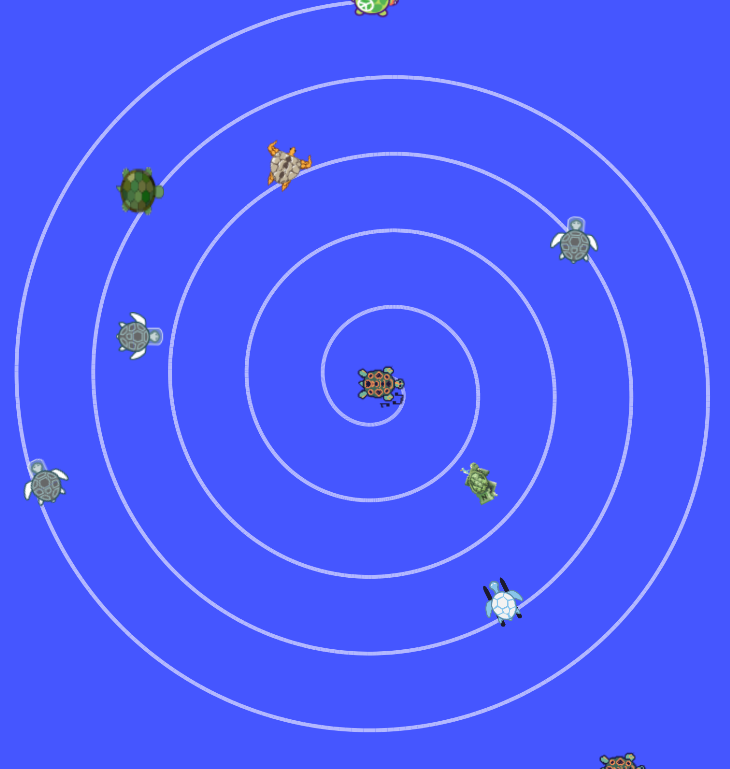
\includegraphics[height=6cm]{Images/03_spawnService.png}
                \caption{Spawning more turtles after drawing a path}
                \label{fig:spawnSrv}
            \end{subfigure}%
            \begin{subfigure}{.5\textwidth}
                \centering
                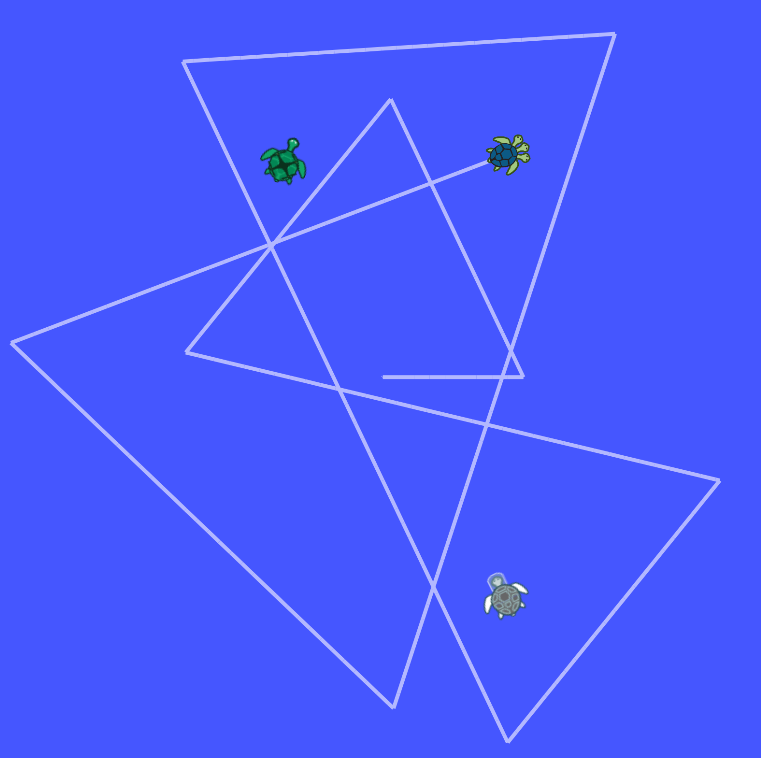
\includegraphics[height=6cm]{Images/03_multiTurtle.png}
                \caption{Drawing a path after spawning multiple turtles}
                \label{fig:multiTurtle}
            \end{subfigure}
            \caption{Spawning service}
    \end{figure}
    
        The results are depicted in Figure \ref{fig:spawnSrv} where the spawn \textit{service} is called multiple times after a turtle has traced a path throughout the canvas, and in Figure \ref{fig:multiTurtle} where the spawn \textit{method} is directly called before animating a turtle. The accomplishment here is that the turtles and the traced path remain on the canvas regardless of the order in which they are generated.
    
    
    \subsection{Path Coloring}
        
        In order to be able to distinguish the turtles on the canvas, it was important to give each turtle its own unique and customizable characteristics such as path color. This was easily accomplished by adding another attribute to the \texttt{Turtle} class. The different path colors can be observed in Figure \ref{fig:pathColor}. Additionally, the canvas color can also be configured during initialization as illustrated in Figure \ref{fig:background}.
        
        \begin{lstlisting}
turtlesim = jupyros.TurtleWidget(background_color="#FFED4A")
turtlesim.turtles["turtle2"].path_color = "#BF0059"
        \end{lstlisting}
        
        
        
    \begin{figure}[hb]
            \centering
            \begin{subfigure}{.5\textwidth}
                \centering
                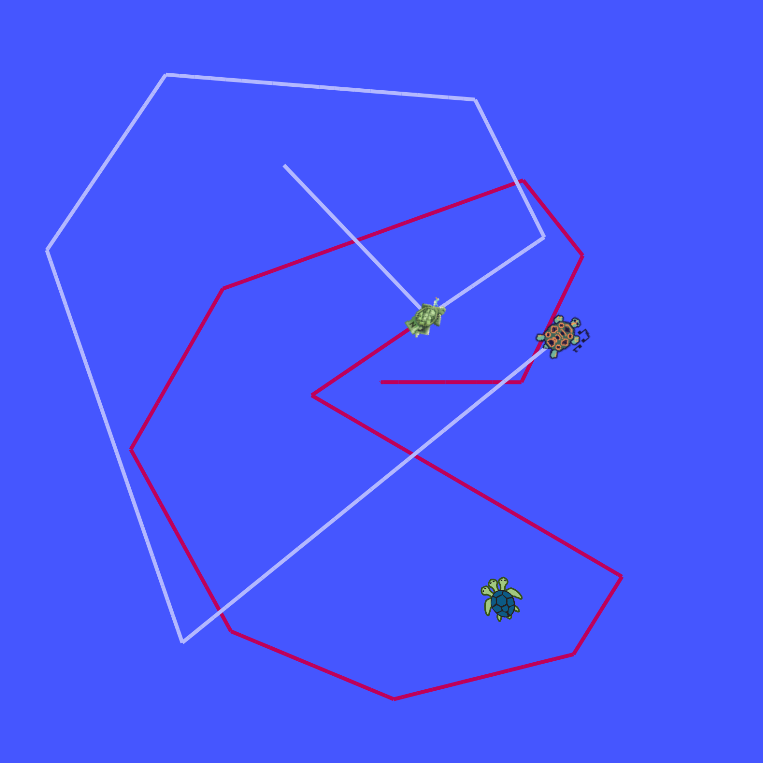
\includegraphics[height=5.8cm]{Images/03_pathColor.png}
                \caption{Customizing the path color of a turtle}
                \label{fig:pathColor}
            \end{subfigure}%
            \begin{subfigure}{.5\textwidth}
                \centering
                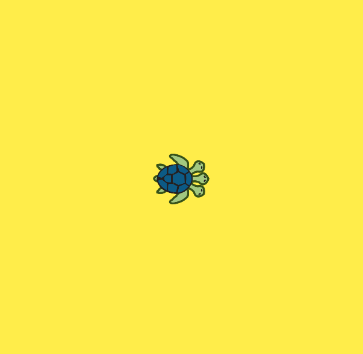
\includegraphics[height=5.8cm]{Images/03_backgroundColor.png}
                \caption{Specifying the background color of the canvas}
                \label{fig:background}
            \end{subfigure}
            \caption{Turtle widget customization}
    \end{figure}
    
        
    
\section{tf2 Transforms}

    \subsection{Follower}
    
        To start introducing navigation into jupyros, the \texttt{turtle\_tf2} tutorial demo was replicated with a canvas animation. This demo uses the tf2 library to broadcast the leading turtle's coordinate frame and to listen for these frames so that the second turtle can compute the differences and chase the first turtle.
    
    \begin{figure}[hb]
        \centering
        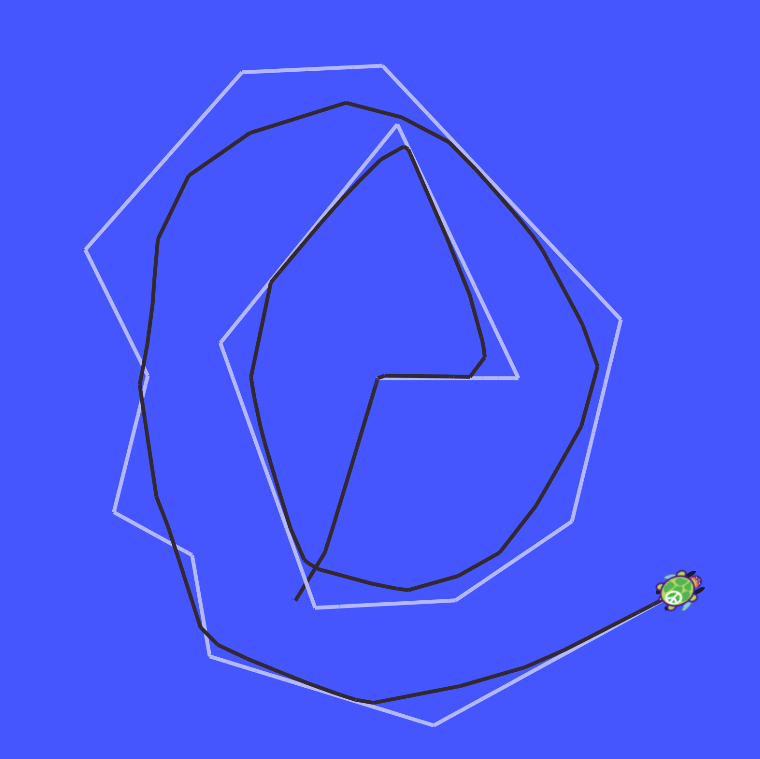
\includegraphics[height=6cm]{Images/03_follower.png}
        \caption{The leading turtle traces the light path while the follower traces the dark path.}
        \label{fig:follower}
    \end{figure}
    
        Several issues were encountered when creating this animation. The biggest hurdle was to update the canvas at the fastest possible rate. However, the \texttt{draw\_image} function takes a short amount of time to draw an image on the canvas; if that time is not provided, the turtle images will not appear on the canvas. To partially alleviate this, the turtle images were stored as canvas objects because they can be drawn quicker on other canvases. As a further remedy, a time counter was integrated into the \texttt{TurtleWidget} class so that the canvas can only be updated every $0.1\ s$. It was determined that this was the shortest amount of time needed two draw both turtles moving.
    
\section{Future Work}

    It would be useful to add examples of how to change a turtle's path color by publishing the specified color to the topic \texttt{/turtle1/color\_sensor}, and to change the background color by adjusting the ROS parameters.

    Also, more content involving the tf2 library needs to be included. The next steps will involve implementing a broadcaster and a listener directly from Jupyter. The ability of Zethus to display transforms needs to be explored as well. And a more elegant solution to the time constraint for drawing images should be implemented, this can potentially be solved from within the ipycanvas library itself.
    
    